% autosam.tex
% Annotated sample file for the preparation of LaTeX files
% for the final versions of papers submitted to or accepted for 
% publication in AUTOMATICA.

% See also the Information for Authors.

% Make sure that the zip file that you send contains all the 
% files, including the files for the figures and the bib file.

% Output produced with the elsart style file does not imitate the
% AUTOMATICA style. The style file is generic for all Elsevier
% journals and the output is laid out for easy copy editing. The
% final document is produced from the source file in the
% AUTOMATICA style at Elsevier.

% You may use the style file autart.cls to obtain a two-column 
% document (see below) that more or less imitates the printed 
% Automatica style. This may helpful to improve the formatting 
% of the equations, tables and figures, and also serves to check 
% whether the paper satisfies the length requirements.

% Please note: Authors must not create their own macros.

% For further information regarding the preparation of LaTeX files 
% for Elsevier, please refer to the "Full Instructions to Authors" 
% from Elsevier's anonymous ftp server on ftp.elsevier.nl in the
% directory pub/styles, or from the internet (CTAN sites) on
% ftp.shsu.edu, ftp.dante.de and ftp.tex.ac.uk in the directory
% tex-archive/macros/latex/contrib/supported/elsevier.


%\documentclass{elsart}               % The use of LaTeX2e is preferred.

\documentclass[twocolumn]{autart}    % Enable this line and disable the 
                                     % preceding line to obtain a two-column 
                                     % document whose style resembles the
                                     % printed Automatica style.


\usepackage{graphicx}          % Include this line if your 
                               % document contains figures,
%\usepackage[dvips]{epsfig}    % or this line, depending on which
                               % you prefer.

\begin{document}

\begin{frontmatter}
%\runtitle{Insert a suggested running title}  % Running title for regular 
                                              % papers but only if the title  
                                              % is over 5 words. Running title 
                                              % is not shown in output.

\title{In Catilinam IV\thanksref{footnoteinfo}} % Title, preferably not more 
                                                % than 10 words.

\thanks[footnoteinfo]{This paper was not presented at any IFAC meeting.}
% \corauth[cor1]{Corresponding author.% R.~Dinkla. Tel. +XXXIX-VI-mmmxxi. Fax +XXXIX-VI-mmmxxv.
% }

\author[TUD]{R. Dinkla\corauthref{cor}}\ead{r.t.o.dinkla@tudelft.nl},    % Add the
\corauth[cor]{Corresponding author.% R.~Dinkla. Tel. +XXXIX-VI-mmmxxi. Fax +XXXIX-VI-mmmxxv.
}
\author[TUD]{S. P. Mulders}\ead{s.p.mulders@tudelft.nl},               % e-mail address 
\author[TUD,TUE]{T. Oomen}\ead{t.a.e.oomen@tudelft.nl},  % (ead) as shown
\author[TUD]{J.W. van Wingerden}\ead{j.w.vanwingerden@tudelft.nl}
\address[TUD]{Delft Center for Systems and Control, Delft University of Technology, Mekelweg 2, 2628CD Delft, The Netherlands}  % Please supply                                              
\address[TUE]{Control Systems Technology Group, Eindhoven University of Technology, 5600
MB Eindhoven, The Netherlands}        % Ful addresses here.

          
\begin{keyword}                           % Five to ten keywords,  
Cicero; Catiline; orations.               % chosen from the IFAC 
\end{keyword}                             % keyword list or with the 
                                          % help of the Automatica 
                                          % keyword wizard


\begin{abstract}                          % Abstract of not more than 200 words.
Cum M.~Cicero consul Nonis Decembribus senatum in aede Iovis 
Statoris consuleret, quid de iis coniurationis Catilinae sociis 
fieri placeret, qui in custodiam traditi essent, factum est, ut 
duae potissimum sententiae proponerentur, una D.~Silani consulis 
designati, qui morte multandos illos censebat, altera C.~Caesaris, 
qui illos publicatis bonis per municipia Italiae distribuendos 
ac vinculis sempiternis tenendos existimabat.
\end{abstract}

\end{frontmatter}
%===============================================================================
% define acronyms here
\begin{acronym}%
    \acro{SPC}{Subspace Predictive Control}
    \acro{DeePC}{Data-enabled Predictive Control}
    \acro{LTI}{linear time-invariant}
    \acro{IV}{instrumental variable}
    \acro{N4SID}{Numerical algorithm for State Space System Identification}
    \acro{MPC}{Model Predictive Control}
\end{acronym}%
%===============================================================================
\section{Introduction}

% \begin{figure}
% \begin{center}
% 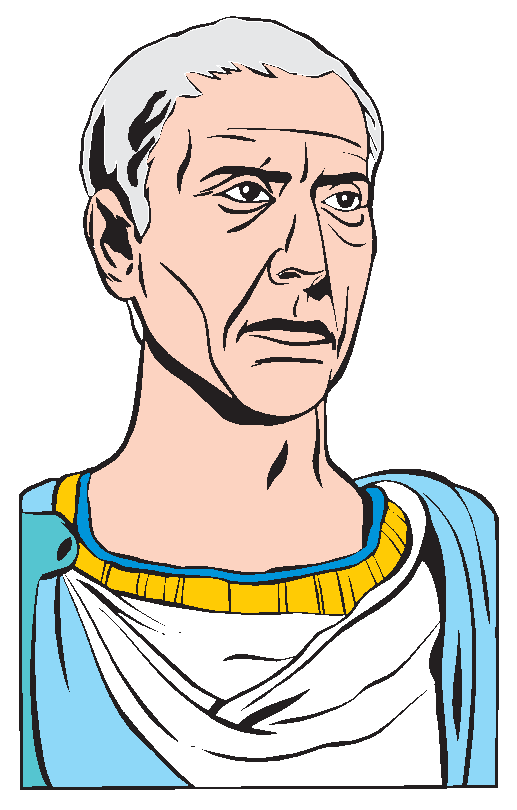
\includegraphics[height=4cm]{jcaesar.eps}    % The printed column  
% \caption{Gaius Julius Caesar, 100--44 B.C.}  % width is 8.4 cm.
% \label{fig1}                                 % Size the figures 
% \end{center}                                 % accordingly.
% \end{figure}

% OR

%\begin{figure}
%\begin{center}
%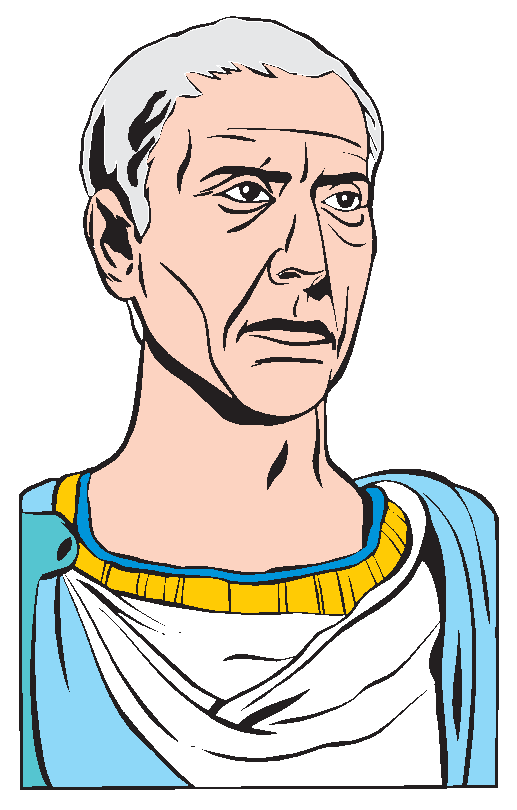
\epsfig{file=jcaesar,width=7cm}
%\caption{Gaius Julius Caesar, 100--44 B.C.}
%\label{fig1}
%\end{center}
%\end{figure}

\subsection{A subsection}
Catiline\footnote{
This footnote should be very brief.}
and for his mastery of Latin prose \cite{Heritage:92}. He was a 
contemporary of Julius Caesar (Fig.~\ref{fig1}).

\section{PRELIMINARIES AND NOTATION}
This section presents the employed system model description and notation that are used throughout this article.

\subsection{SYSTEM MODEL}
A typical generic, non-deterministic discrete \ac{LTI} system considers both process and measurement noise
\begin{subequations}\label{eqn:SS_wv}
\begin{align}
	\bar{x}_{k+1} &= A\bar{x}_k + Bu_k + w_k,\label{eqn:SSwv_x}\\
	y_k &= C\bar{x}_k + Du_k + v_k \label{eqn:SSwv_y},
\end{align}
\end{subequations}
in which ${\bar{x}_k\in\mathbb{R}^n}$, ${u_k\in\mathbb{R}^r}$, ${y_k\in\mathbb{R}^l}$, ${w_k\in\mathbb{R}^n}$, ${v_k\in\mathbb{R}^l}$, respectively are states, inputs, outputs, process noise, and measurement noise at the time instant denoted by the subscript $k$. In addition, $A$, $B$, $C$, $D$ respectively are the state transition, input, output, and direct-feedthrough matrices of corresponding dimensions.

Let the process and measurement noise be zero-mean random sequences with covariance matrix
\begin{equation*}
    \mathbb{E}\left\{\begin{bmatrix}w_k\\v_k\end{bmatrix}\begin{bmatrix}w_j^\top & v_j^\top\end{bmatrix}\right\} =
\begin{bmatrix}Q & S\\S^\top & R\end{bmatrix}\delta_{kj},
\end{equation*}
in which $R>0$, $\delta_{kj}$ is the Kronecker delta function (1 if $k=j$, 0 otherwise). If the covariance matrix above, before $\delta_{kj}$, is positive semi-definite, the pair $(A,\,C)$ is observable, and $(A,\,Q^{1/2})$ is reachable, then there exists an innovation form representation that is equivalent to~\eqnref{eqn:SS_wv} given by~\cite[p.~\todo{Find pages}]{Anderson1979}, \cite[p.~162]{Verhaegen2007a}%
\begin{subequations}\label{eqn:SS_innovation}
\begin{align}
	x_{k+1} &= Ax_k + Bu_k + Ke_k,\label{eqn:SSi_x}\\
	y_k &= Cx_k + Du_k + e_k \label{eqn:SSi_y},
\end{align}
\end{subequations}
in which $x_k\in\mathbb{R}^{n}$ represents states (different from $\bar{x}_k$), $e_k$ represents so called innovation noise, and $K\in\mathbb{R}^{n\times l}$ is a constant Kalman gain matrix that renders ${\tilde{A}=A-KC}$ asymptotically stable. By substituting \eqnref{eqn:SSi_y} into \eqnref{eqn:SSi_x} one alternatively obtains the equivalent predictor form
\begin{subequations}\label{eqn:SS_innovation}
\begin{align}
	x_{k+1} &= \tilde{A}x_k + \tilde{B}u_k + Ky_k,\label{eqn:SSp_x}\\
	y_k &= Cx_k + Du_k + e_k \label{eqn:SSp_y},
\end{align}
\end{subequations}
in which $\tilde{B}=B-KD$.

\subsection{Notation}
Having described the different representations of the considered discrete, non-deterministic \ac{LTI} systems, this section introduces the notation used in this work.

To start, a block-Toeplitz matrices are defined by
\begin{align}\label{eqn:blockToeplitz} 
\mathcal{T}_s(\mathcal{A},\mathcal{B},\mathcal{C},\mathcal{D}) =\scriptsize{
	\begin{bmatrix}
		\mathcal{D}         & 0         & 0      & \cdots  & 0\\
		\mathcal{C}\mathcal{B}        & \mathcal{D}         & 0      & \cdots  & 0\\
		\mathcal{C}\mathcal{A}\mathcal{B}       & \mathcal{C}\mathcal{B}        & \mathcal{D}      & \cdots & 0\\
		\vdots    &  \vdots & \ddots & \ddots & \vdots\\
		\mathcal{C}\mathcal{A}^{s-2}\mathcal{B} & \mathcal{C}\mathcal{A}^{s-3}\mathcal{B} & \cdots  & \mathcal{C}\mathcal{B}     & \mathcal{D}
	\end{bmatrix}},
\end{align}
in which the subscript $s$ indicates the number of block-rows, and the matrices $\mathcal{A}$, $\mathcal{B}$, $\mathcal{C}$, and $\mathcal{D}$ are all of compatible dimensions. Let $I_s\in\mathbb{R}^{s\times s}$ represent an identity matrix and $f\in\mathbb{Z}^+$ a strictly-positive integer prediction window length. Equation~\eqnref{eqn:blockToeplitz} thereby defines the block-Toeplitz matrices
\begin{alignat*}{2}
\Tf{u}&=\mathcal{T}_f(A,B,C,D),\quad  &\Hf&=\mathcal{T}_f(A,K,C,I_l),\\
\tTf{u}&=\mathcal{T}_f(\tilde{A},\tilde{B},C,D),\quad  &\tHf&=\mathcal{T}_f(\tilde{A},K,-C,I_l).
\end{alignat*}

In addition, two extended observability matrices are defined by
\begin{align*}
\Gf &= \begin{bmatrix}C^\top & (CA)^\top & \cdots & (CA^{f-1})^\top\end{bmatrix}^\top\quad\text{and}\\
\tGf &= \begin{bmatrix}C^\top & (C\tilde{A})^\top & \cdots & (C\tilde{A}^{f-1})^\top\end{bmatrix}^\top,
\end{align*}
and two extended reversed controllability matrices are defined as 
\begin{align*}
\tKp{u} &= \begin{bmatrix} \tilde{A}^{p-1}\tilde{B}\:\, & \tilde{A}^{p-2}\tilde{B} & \cdots & \tilde{A}\tilde{B} & \tilde{B}\:\, \end{bmatrix},\text{ and}\\
\tKp{y} &= \begin{bmatrix} \tilde{A}^{p-1}K & \tilde{A}^{p-2}K & \cdots & \tilde{A}K & K \end{bmatrix}.
\end{align*}

Furthermore, data vectors are denoted as examplified by
\begin{align*}
    \datavec{y}{i,p} = \begin{bmatrix} y_i^\top & y_{i+1}^\top & \cdots & y_{i+p-1}^\top\end{bmatrix}^\top,
\end{align*}
which represents a vector of ordered output data starting at the time index given by the first subscript $i$, and containing a number of data samples indicated by the second subscript $p$. Akin to $f$, the subscript $p\in\mathbb{Z}^+$ will be used throughout this work to refer to a strictly-positive integer that represents a certain window length of data.

Using such data vectors it is possible to concisely define block-Hankel data matrices. Such a block-Hankel data matrix is examplified by
\begin{align*}
    Y_{i,p,N} = \begin{bmatrix}
        \datavec{y}{i,p} & \datavec{y}{i+1,p} & \cdots & \datavec{y}{i+N-1,p}
    \end{bmatrix},
\end{align*}
which contains $N\in\mathbb{Z}^+$ successive output data vectors with $p$ data samples each, starting from time index $i$.

\section{The argument}
Some words might be appropriate describing equation~(\ref{e1}), if 
we had but time and space enough.
\begin{equation} \label{e1}
{{\partial F}\over {\partial t}} =
D{{\partial^2 F}\over {\partial x^2}}.
\end{equation}
See \cite{Abl:56}, \cite{AbTaRu:54}, \cite{Keo:58} and 
\cite{Pow:85}.
This equation goes far beyond the celebrated theorem ascribed to the great
Pythagoras by his followers.
\begin{thm}
The square of the length of the hypotenuse of a right triangle equals the sum of the squares 
of the lengths of the other two sides.
\end{thm}
\section{Epilogue}
A word or two to conclude, and this even includes some inline 
maths:  $R(x,t)\sim t^{-\beta}g(x/t^\alpha)\exp(-|x|/t^\alpha)$.

\begin{ack}                               % Place acknowledgements
Partially supported by the Roman Senate.  % here.
\end{ack}

\bibliographystyle{plain}        % Include this if you use bibtex 
\bibliography{autosam}           % and a bib file to produce the 
                                 % bibliography (preferred). The
                                 % correct style is generated by
                                 % Elsevier at the time of printing.

\appendix
% \section{A summary of Latin grammar}    % Each appendix must have a short title.
% \section{Some Latin vocabulary}         % Sections and subsections are supported  
                                        % in the appendices.
\end{document}